\section{Einführung}
\paragraph{It's okay}

\begin{figure}[H]
	\centering
	
\includegraphics[scale = 0.3]{attachment/chapter_OWN/Scc004}
\end{figure}
Nicht jede Idee muss gleich zu Ende geführt werden. 

\paragraph{How to start}

\begin{figure}[H]
	\centering
	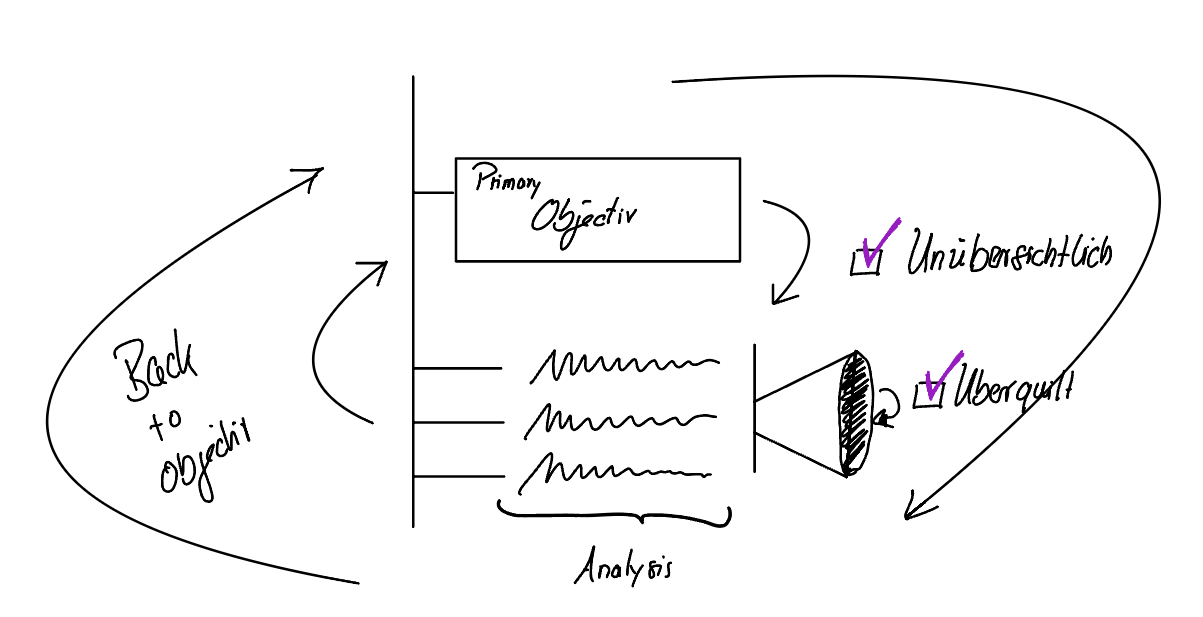
\includegraphics[scale = 0.3]{attachment/chapter_OWN/Scc003}
\end{figure}


Ein generelles Prinzip (Integration!)
\begin{enumerate}
	\item Der Aufbau sollte so sein, dass das Primary Objective an erster Stelle steht. Mein persönliches Risiko ist, dass ich zu viel Zeit in die Analyse setzte. Am Ende bleibt dann kaum noch Zeit für ein „Refaktoring“.
	\item Bis es überquillt - Zu erst soll solange im oberen Kapitel geschrieben werden, bis es „unübersichtlich“ wird, sodass ein Auslagern sinnvoll ist. - Immer etwas zu lange warten.
	\item Wenn ich in der Analyse bin, sollte hier mögliche Kategorien nach Nutzen aufgesetzte werden. - Es sollen Kategorien immer etwas zu spät gebildet werden. Das persönliche Risiko wird dahingegen mindert, dass der Zeitaufwand für das Testen der Kategorie höher sein soll, als die Konzeption.
	\item Back to Objective: Ist das Objective im Blick, kann die Analyse abgeschlossen werden, wenn mit dem Abschluss, dass Objective weiter verfolgen zu können. - Ware Motivation. 
\end{enumerate}